\documentclass[./\jobname.tex]{subfiles}
\begin{document}

\chapter{Task Description}

This project is about simulating and optimising a circulative traffic light control. The simulation is done with  \href{https://www.dlr.de/ts/en/desktopdefault.aspx/tabid-9883/16931_read-41000/}{SUMO} which stands for Simulation of Urban MObility. SUMO provides an API that allows external programs to cast and control a simulation. These control structures, simulation evaluation as well as the optimisation algorithms are programmed in Python 3.7. \\~\\
The project includes the following tasks: 
\begin{itemize}
	\item create infrastructure to call simulation and alter simulation parameters in SUMO
	\item construct different intersections at different traffic loads
	\begin{itemize}
		\item Manhattan grid layout: 3x3
		\item traffic load: night, day
	\end{itemize}
	\item four different optimisation algorithms
	\begin{itemize}
		\item NSGA2
		\item Conjugate Gradient Descent
		\item Differential Evolution
		\item self-created heuristic using Hill-Climbing
	\end{itemize}
	\item description and evaluation of the results
	\item precise technical report to ensure repeatability 
\end{itemize}

The simulation returns three parameters: 
\begin{itemize}
	\item overall waiting time calculated as the mean waiting time per car
	\item overall number of stops calculated as the sum of the stops by all cars
	\item fairness in waiting time calculated as the variance of the waiting times \\
\end{itemize}
We are looking for a solution that minimises all of these parameters. \\
All of the considered traffic load scenarios are stable. This means, that, under the condition that the optimisation algorithm does not generate impracticable results, the waiting line does not grow arbitrarily large. 

\newpage



\chapter{Scenarios}
This chapter is about creating the problem-scenarios in sumo. As stated in the task description, two scenarios on a 3x3 Manhattan gird with different traffic loads for day and night are created. 


\section{Street Network}

We used a 3x3 street network for the following simulations.

\begin{figure}[H]
	\centering
	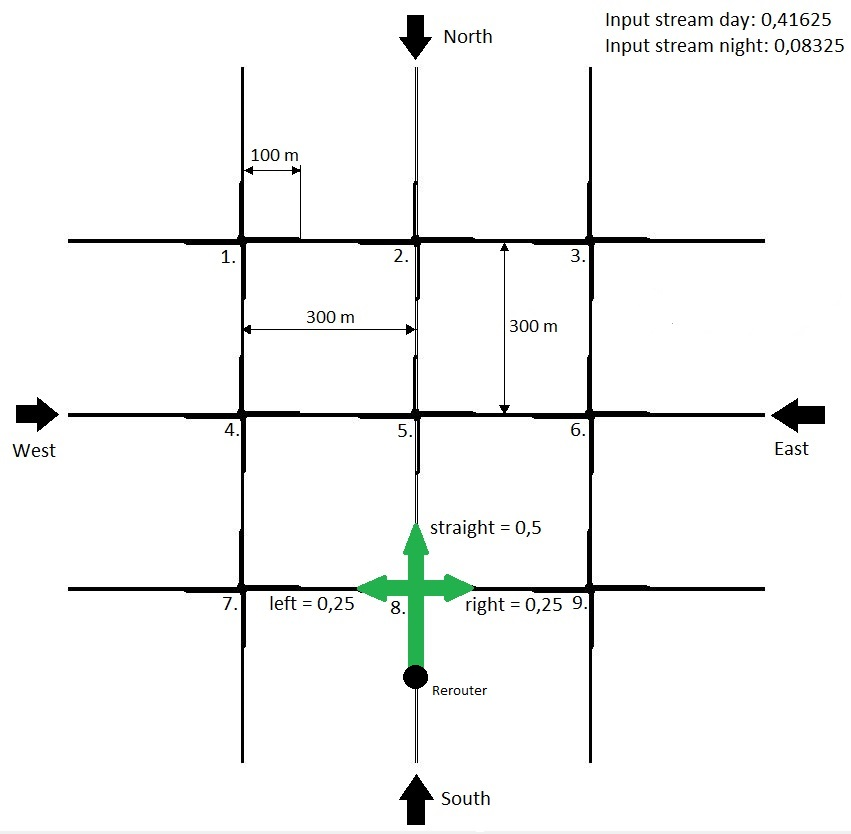
\includegraphics[width=0.75\linewidth]{../img/jpg/3x3_inf.jpg}
	\caption{3x3 street network}
	\label{fig:3x3inf}
\end{figure}

The street network can be seen in figure \ref{fig:3x3inf}. Only one inflow from each direction (see black arrows) is defined. Rerouters are used for all intersections, which are provided by sumo (see green arrow). The rerouter is implemented with the following turn probability's left 0.25, right 0.25 and straight 0.5.



\section{Traffic Load}

The traffic load is calculated using the programs Streetnetwork and LPsolve. This is done under the assumption, that the traffic behaves like a fluid (continuous simulation). First the network is created using the program Streetnetwork.

\begin{figure}[H]
	\centering
	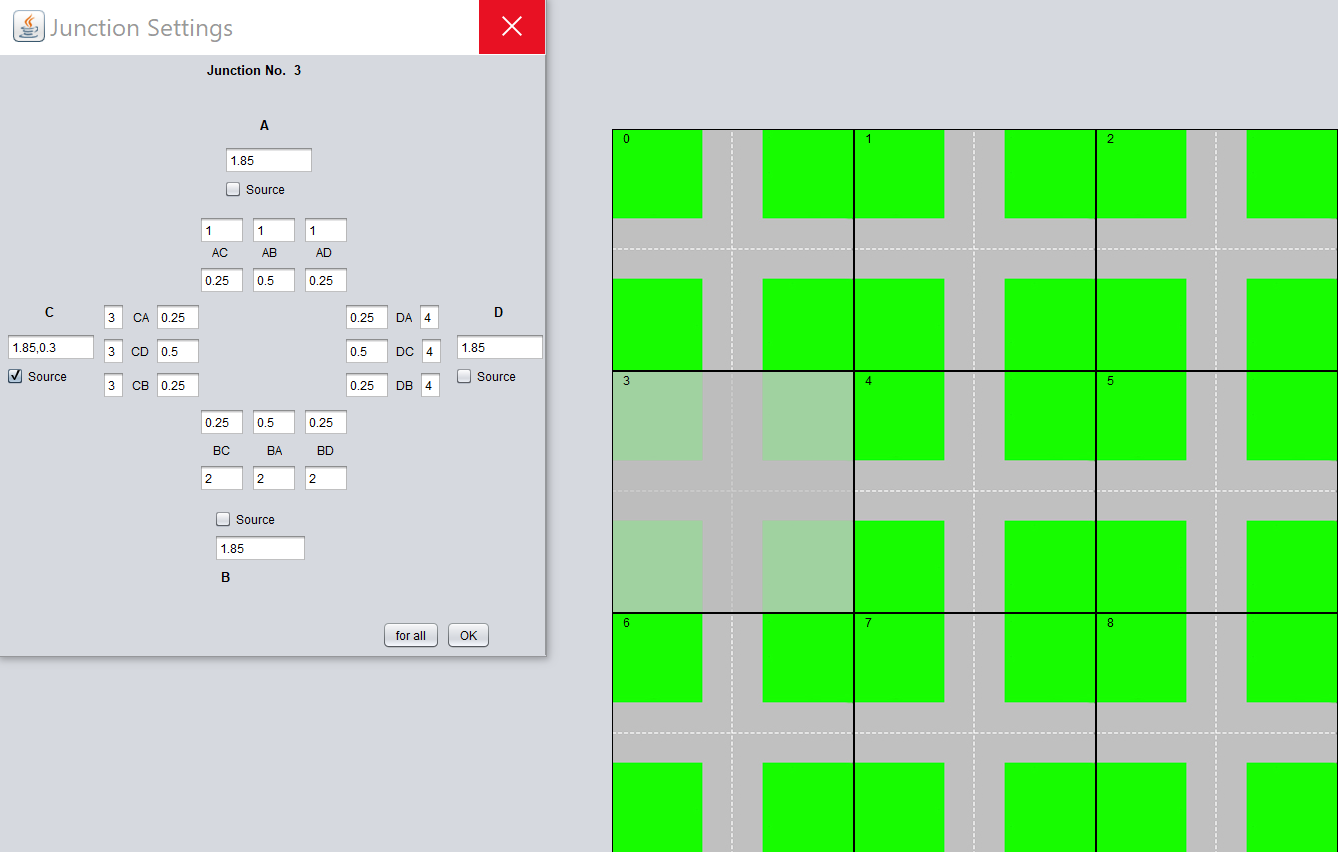
\includegraphics[width=0.9\linewidth]{../img/png/StreetNetworker.png}
	\caption{creation of street network}
	\label{fig:stret_net}
\end{figure}

Figure \ref{fig:stret_net} shows the creating process. All inflow values are set to the value 0.3 and all outflow values are set to the value 1.85. We defined a day ($\epsilon$ = 0.5) and a night ($\epsilon$ = 0.9) scenario. The program then crates a script, which can be used in LPsolve for the calculation of the c value.

\begin{figure}[H]
	\centering
	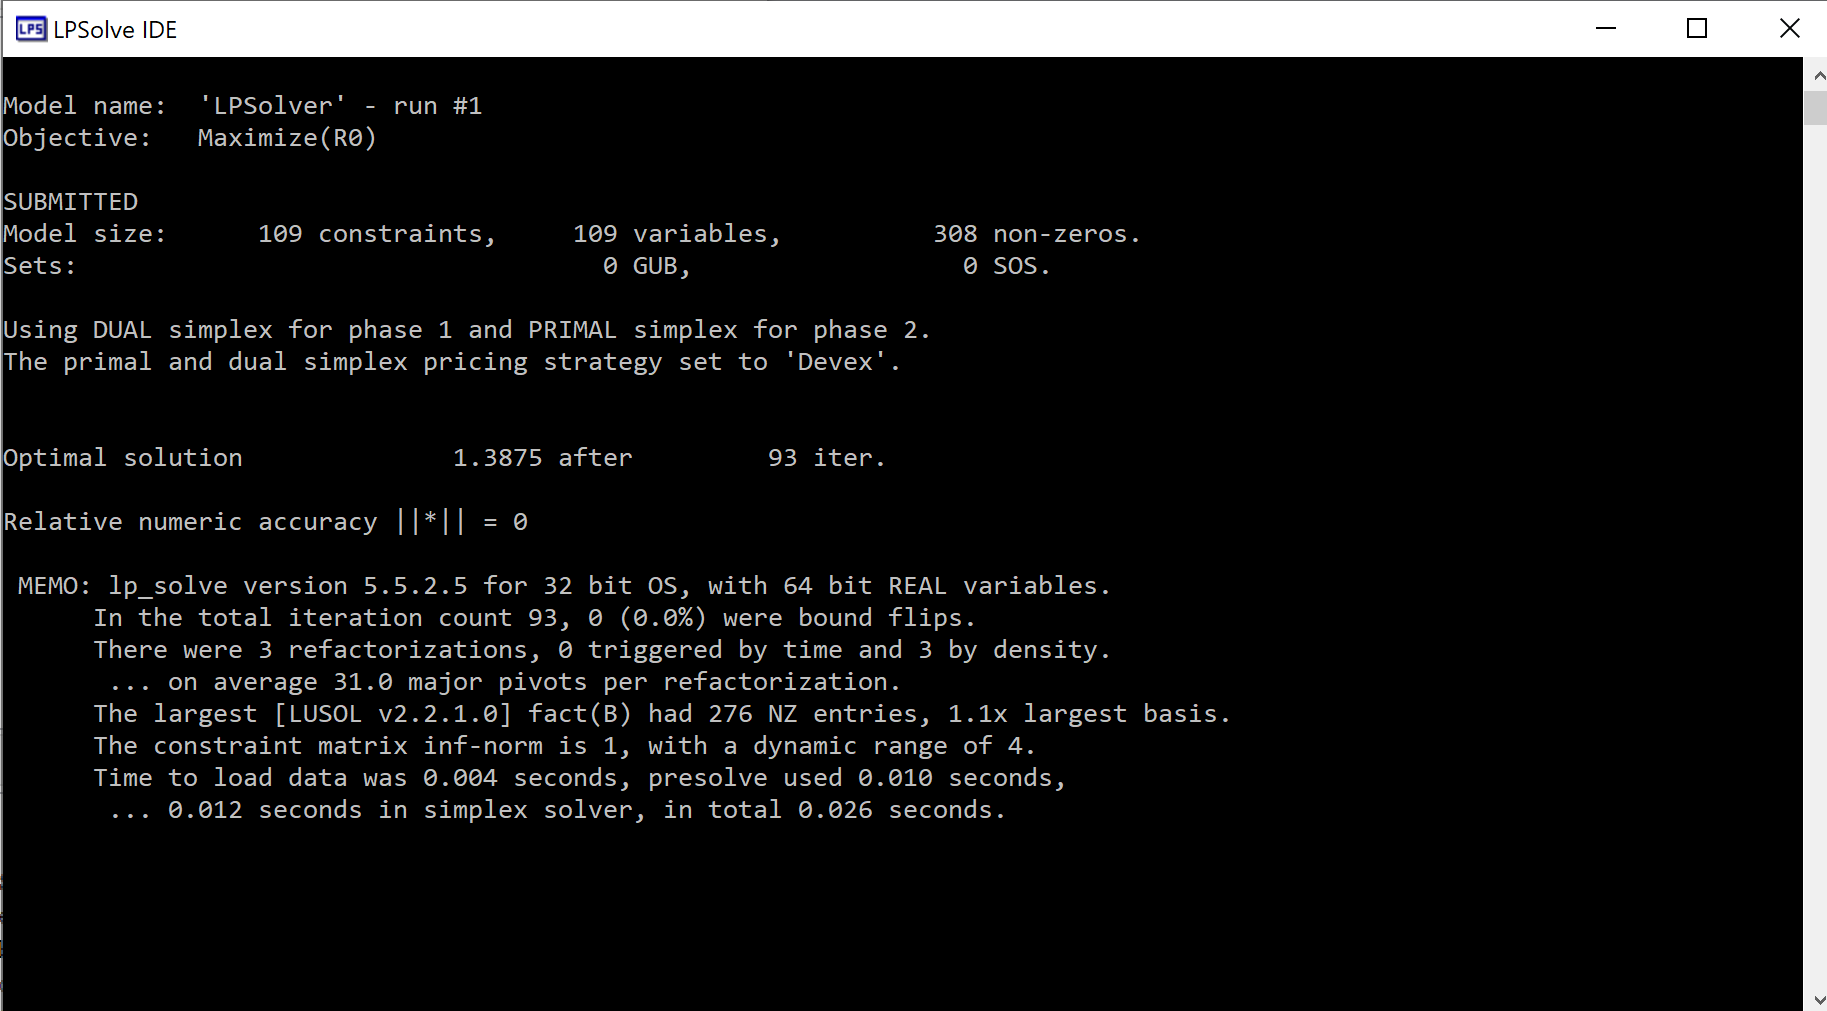
\includegraphics[width=0.8\linewidth]{../img/png/epsilon05.png}
	\caption{calculation with $\epsilon = 0.5$}
	\label{fig:epsilon05png}
\end{figure}

\begin{figure}[H]
	\centering
	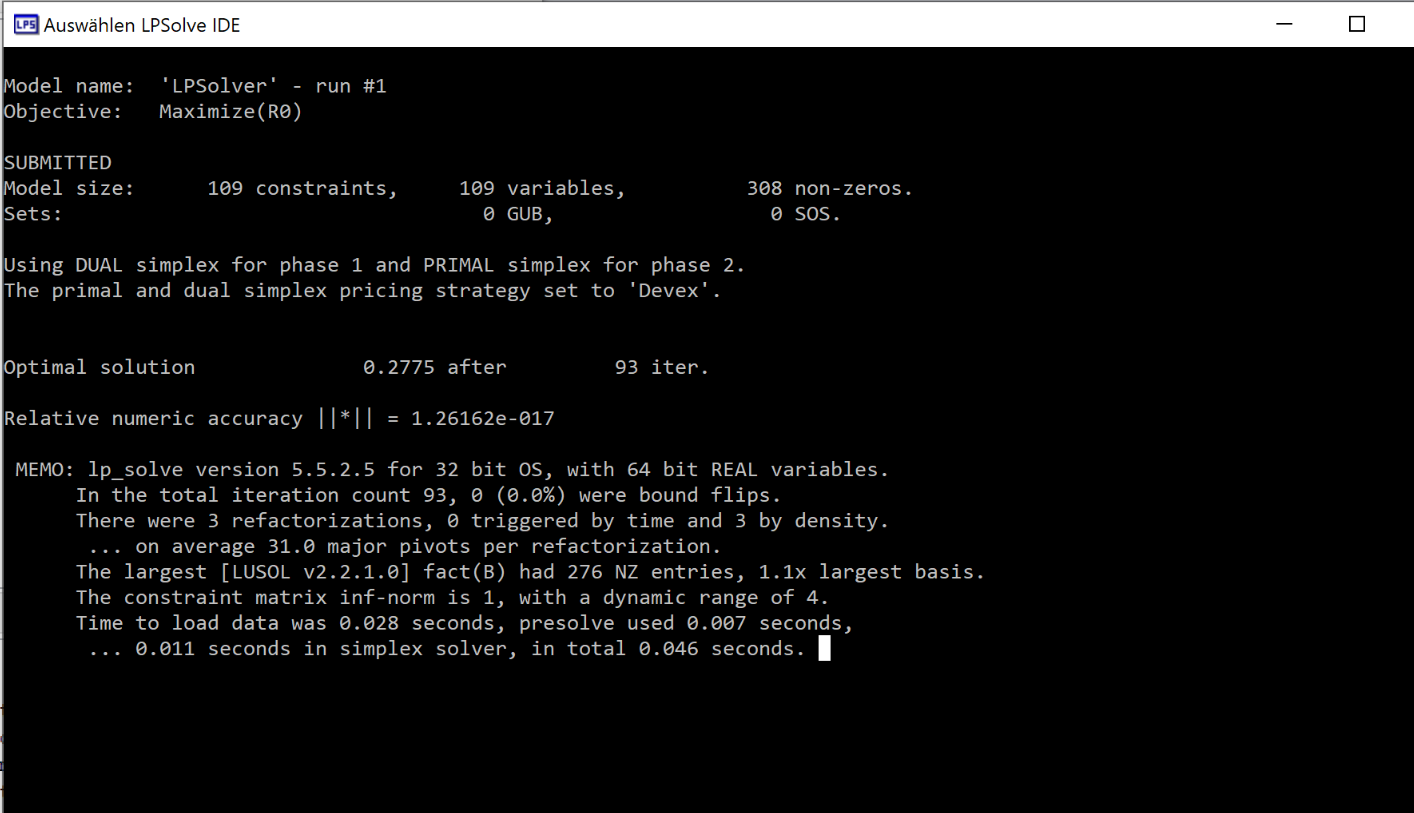
\includegraphics[width=0.8\linewidth]{../img/png/epsilon09.png}
	\caption{calculation with $\epsilon = 0.9$}
	\label{fig:epsilon09}
\end{figure}

Figure \ref{fig:epsilon05png} and figure \ref{fig:epsilon09} show the output of for the c values calculated with LPsolve. The used inflow values for day 0.41625 and night 0.08325 are then calculated by multiplying the chosen inflow value (0.3) with the calculated c values. 



\section{Calculate Relative Green}

The following image \ref{fig:greenphases} shows the green phases for each intersection.

\begin{figure}[H]
	\centering
	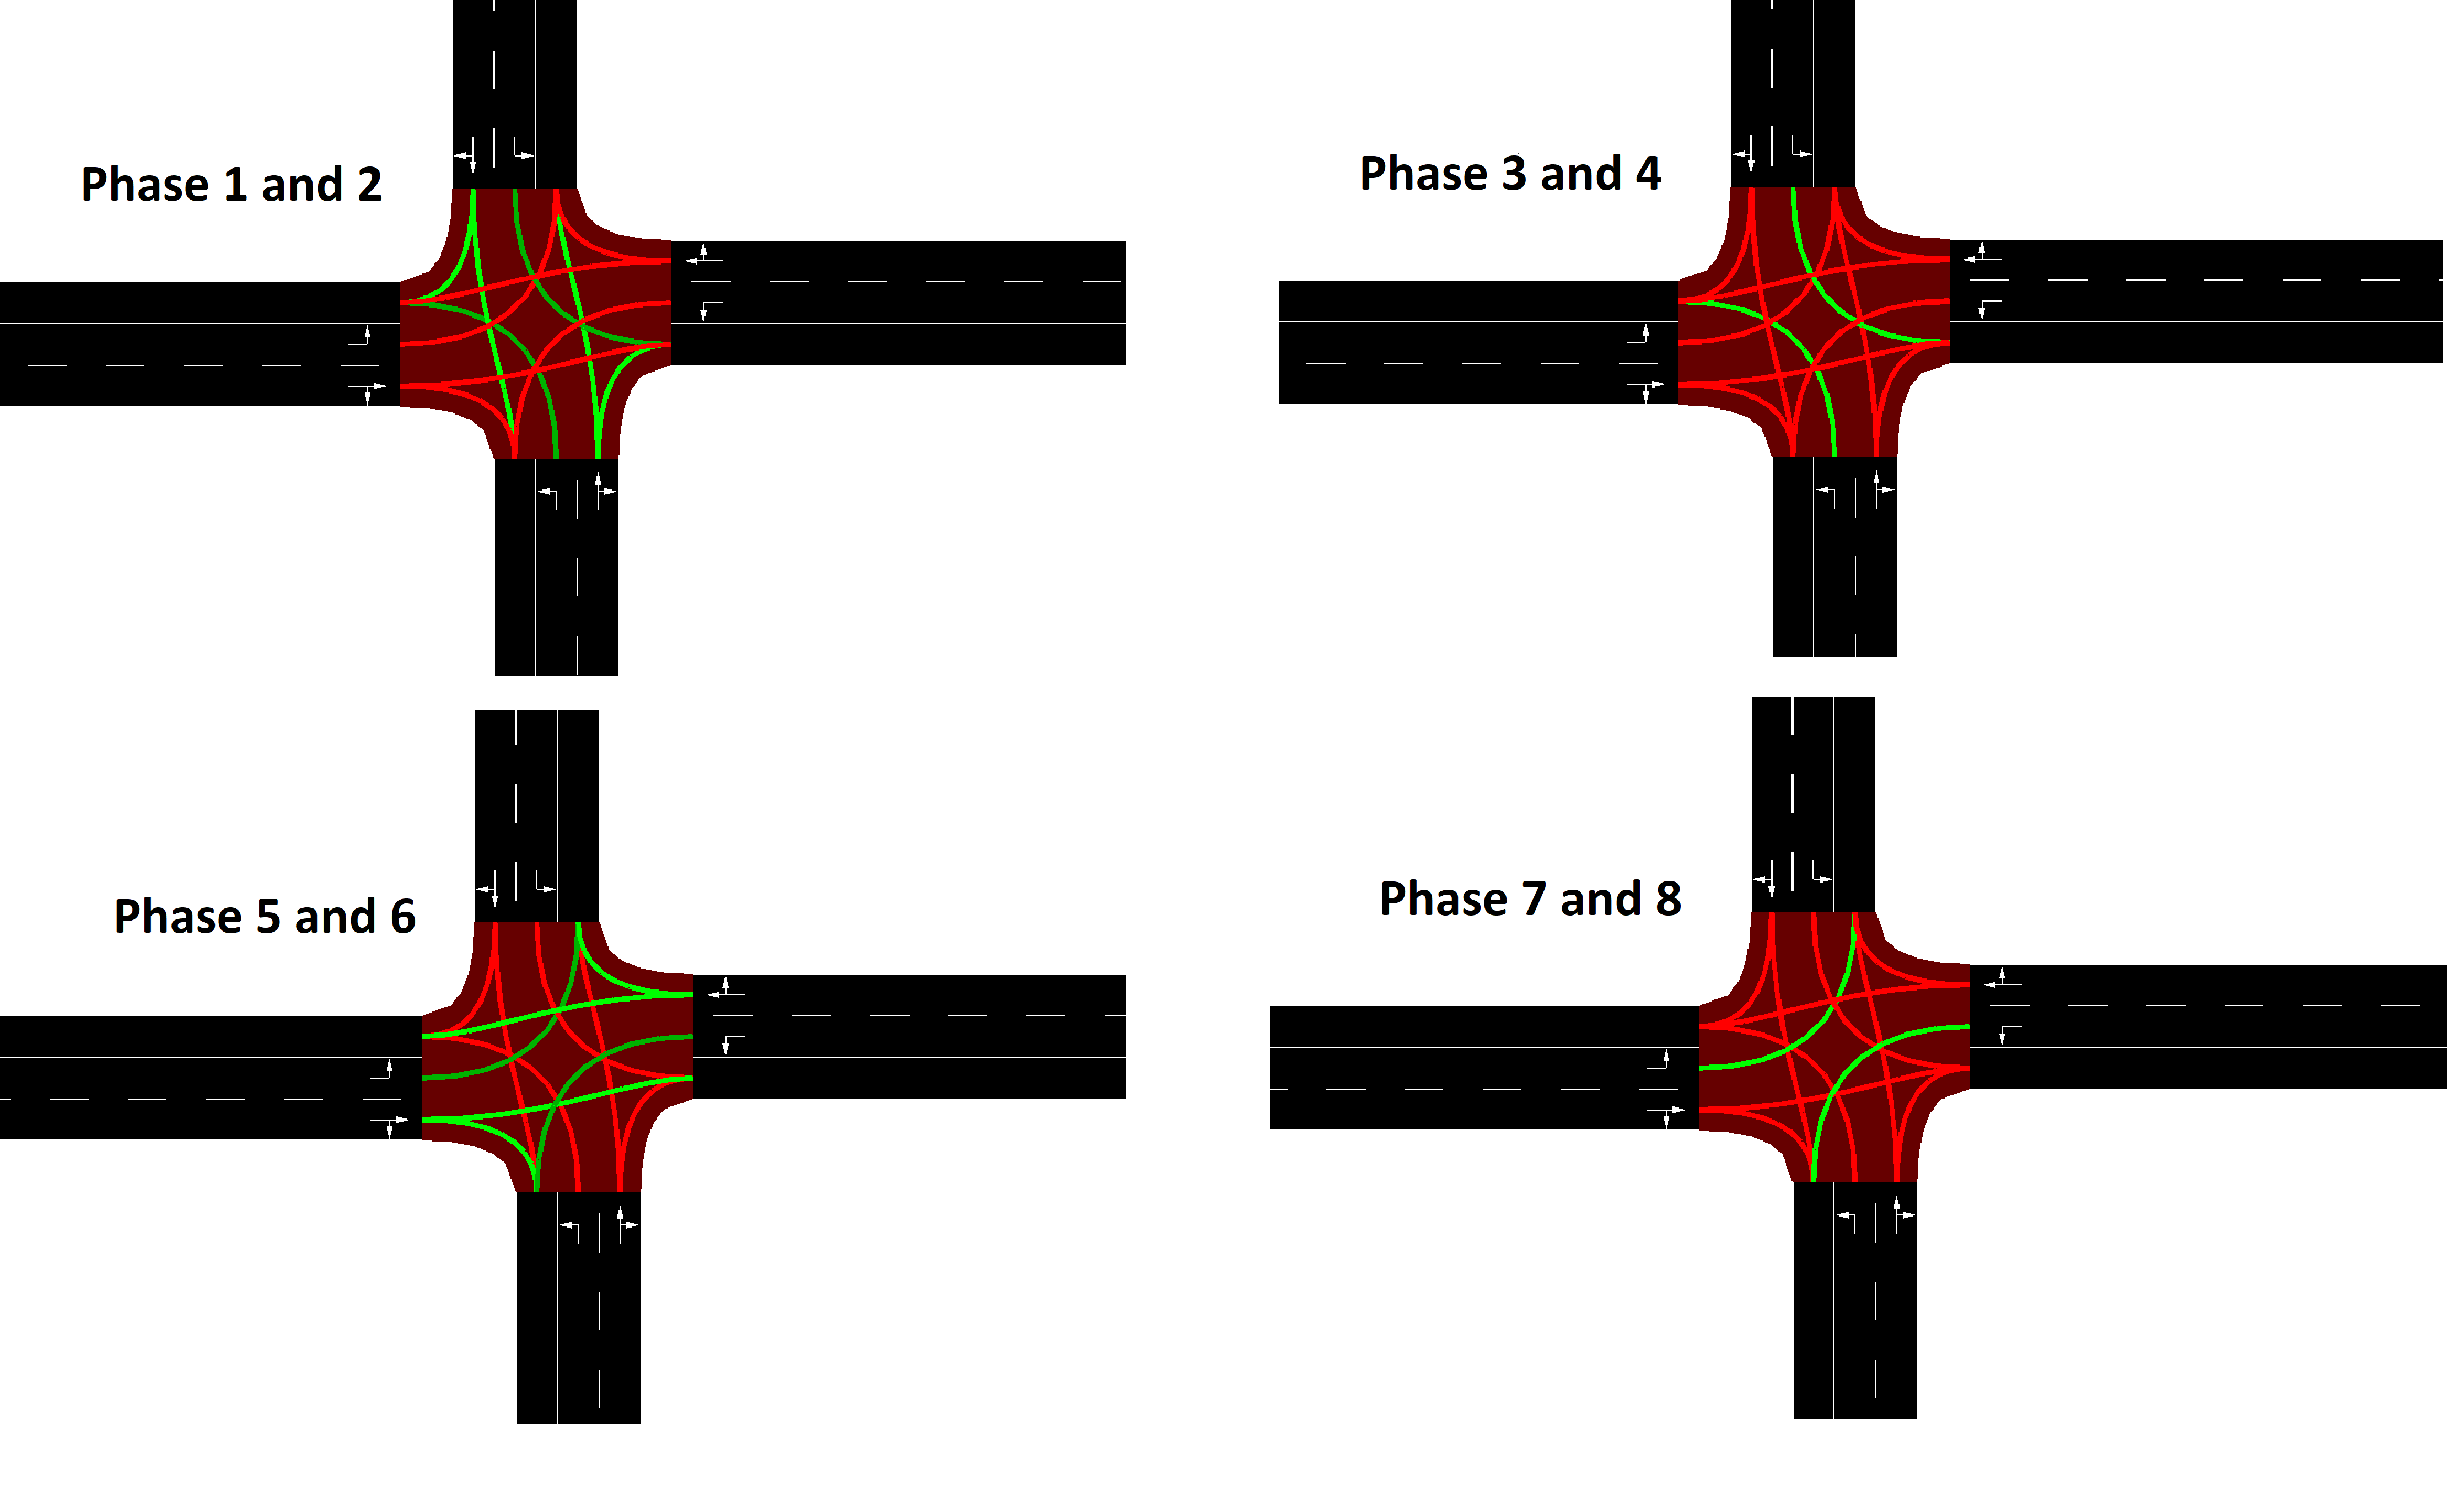
\includegraphics[width=1\linewidth]{../img/png/cross_phases.png}
	\unterschrift{traffic light phases for each intersection}{}{}
	\label{fig:greenphases}
\end{figure}

The calculation of the relative greens phases is related to the input stream into the intersection. If we call the input stream from the street i $I_{i}$ and the turn probability from the i-th street to the j-th street $p_{ij}$, then we can determine the relative green time using an weighted average. Note that the streets are numerated from 1 (north) increasing clockwise to 4 (west). For the first relative green time (seen in figure \ref{fig:greenphases}, upper left corner) we get the following calculation:

\begin{equation}\label{key}
rg_{phase 1} = \frac{max(I_{1}(p_{13} + p_{14})+I_{3}(p_{31}+p_{32}))}{\sum_{i=1}^{4}phase_{i}} 
\end{equation}

This is because, the input stream from street 1 divided (according to the turn probabilities) into street 3 ($I_{1}p_{13}$) and street 4 ($I_{1}p_{14}$). The same is done for the input stream $I_{3}$. Then this value is divided by the sum of all green phases. This procedure is then used to calculate all four phases.



\chapter{Algorithms}
This chapter describes the pseudocode and the characteristics of the implemented optimisation algorithms. Altogether four different optimisers are compared: Differential Evolution (DE), Non Dominated Sorting Genetic Algorithm (NSGA II), Conjugate Gradient Descent (CGD) and a self-created heuristic based on the Hill-Climbing (HC) principal. All optimiser have been tested to work on deterministic multidimensional sphere functions. The table \ref{tab:sphere} shows the implementation of this testfunction in 2D space. Since the NSGA-II is designed for multicriteria optimisation, the testfunction must be adapted: two overlapping spheres are optimised. 

\begin{table}[H]
	\centering
	\noindent\adjustbox{max width=\linewidth}{
		\begin{tabular}{|c|c|}
			\hline \\
			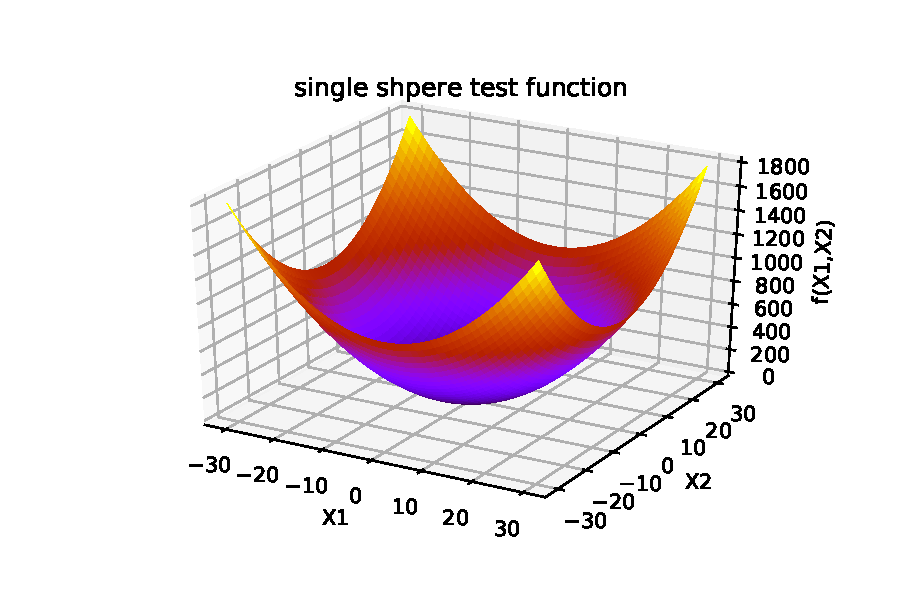
\includegraphics[width=\textwidth]{../img/pdf/singleSphere.pdf} &
			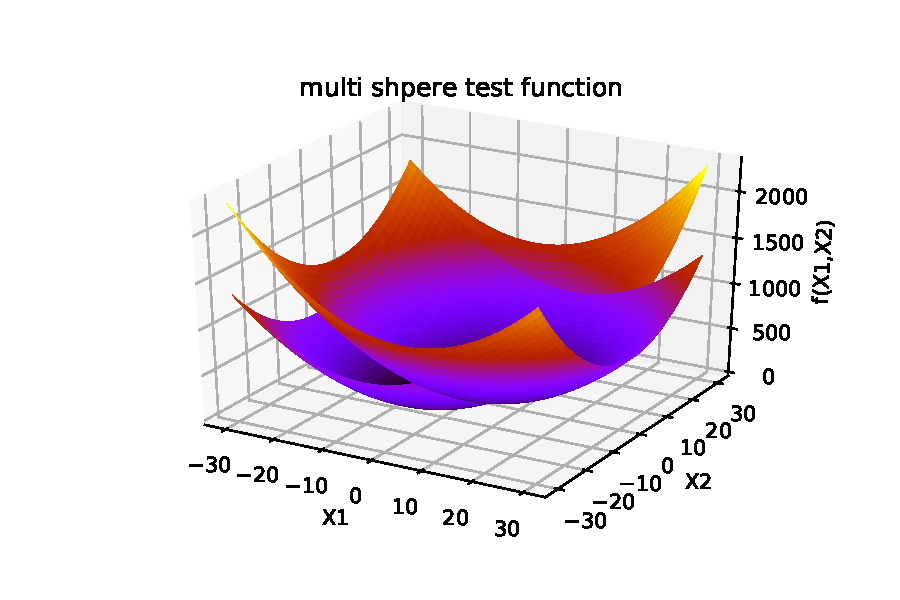
\includegraphics[width=\textwidth]{../img/pdf/multiSphere.pdf} \\
			\hline
		\end{tabular}
	}
	\unterschrift{comparison of single-criteria and multi-criteria sphere function}{}{}
	\label{tab:sphere}
\end{table}


\section{Differential Evolution}

Differential Evolution was first published by \cite{storn_differential_1997}. New forms and adaptions are constantly developed which belong to some of the best performing optimisation algorithms. The "framework" of Differential Evolution is described in \autoref{algo: DE}. 

\begin{algorithm}
	\SetAlgoNoLine
	\DontPrintSemicolon
	population $\gets$ initialization\;
	\While{g < $G_{max}$}{
		\For {individual $x_i$ \textbf{in} population} {
			$v_i$ = muation($x_i$, population, F)\;
			$u_i$ = crossover($x_i$, $v_i$, CR)\;
			\If {function($u_i$) < function($x_i$)} {
				$x_i$ = $u_i$\;
			}
		}
		g = g + 1\;
	}
	\unterschrift{Differential Evolution}{}{}
	\label{algo: DE}
\end{algorithm}

The framework allows for different definitions of mutation and crossover. In this implementation the mutation $rand\textunderscore1$ is used. The following equation \ref{eq: mutation rand 1} describes this mutation operator. The subscript $i$ hereby stands for the current individual in the loop. The indices $r1$ to $r3$ denote random but different individuals in the population. 

\begin{equation}
\label{eq: mutation rand 1}
v_i = x_{r1} + F (x_{r2} - x_{r3})
\end{equation}

The parameter $F$ is also called the scalefactor and can be chosen by the user. Typically this is set to be a number in the intervall $F = \left[ 0 ... 1 \right] $.

Further a binomial crossover strategy is used. For every coordinate $j$ in the vector, either an element of the old vector $x_i$ or a new vector $v_i$ is chosen. This again depends on a user defined parameter $CR$ called the crossover rate. To ensure, that at least on single element from the new vector is chosen, a random coordinate $K$ must be transferred. 

\begin{equation}
u_{ij}=\begin{cases}
v_{ij}, &\text{if $j = K \lor rand[0,1] \leq CR$}\\
x_{ij}, &\text{otherwise}
\end{cases}
\end{equation}

The following figure \ref{fig:de_verification} shows the verification of the differential evolution algorithm on the sphere function. 

\begin{figure}[H]
	\centering
	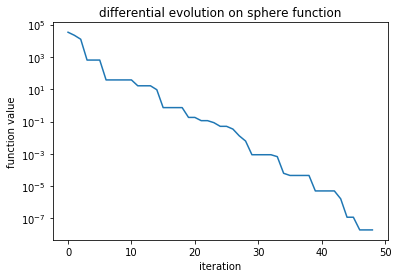
\includegraphics[width=0.9\linewidth]{../img/png/differential_evolution_varification.png}
	\caption{testrun of differential evolution on the sphere, shows how the function value depends on the iteration}
	\label{fig:de_verification}
\end{figure}

\section{Nondominated Sorting Genetic Algorithm II}
The NSGA-II was proposed by Kalyanmoy \cite{deb_fast_2002}. In contrary to the DE, this algorithm is able to optimise multiple functions at the same time. This is called a multi-criteria optimiser. The result of this algorithm are multiple individuals in a population. Ideally this population describes the pareto front. These are all feasible solutions, the user can then decide which optima is best suited for that specific application. \\

The implementation was done in conjunction with the algorithm description in appendix \ref{chap: NSGA2_Description}. For a more convenient implementation and readability, every individual in the NSGA II is an object of the class \textit{individual} which holds the most important attributes of a candidate. The following pseudocode \ref{algo: NSGA2} outlines the general steps to perform the NSGA II algorithm. 

\begin{algorithm}[H]
	\SetAlgoNoLine
	\DontPrintSemicolon
	population $\gets$ initialization\;
	\While{g < $G_{max}$}{
		\For {i \textbf{in} population/2} 
		{
			$p1$, $p2$ = tournament\textunderscore selection(Pt)\;
			$q1$, $q2$ = crossover($p1$, $p2$)\;
			$q1$ = mutation($q1$)\;
			$q2$ = mutation($q1$)\;
			Qt = Qt $\cup$ ($q1$, $q2$)\;
		}
		Rt = Rt $\cup$ (Qt)\;
		Rt = fast\textunderscore non\textunderscore dominated\textunderscore sort(Rt)\;
		Pt = crowding\textunderscore distance\textunderscore sorting(Rt, Pt.size)\;
		g = g + 1\;
	}
	\unterschrift{NSGA II}{}{}
	\label{algo: NSGA2}
\end{algorithm}


Figure \ref{fig:nsga2_verification} describes a simple testrun of the algorithm on a multi-criteria sphere function. The plot clearly shows that the algorithm is able to find a valid pareto front. 

\begin{figure}[H]
	\centering
	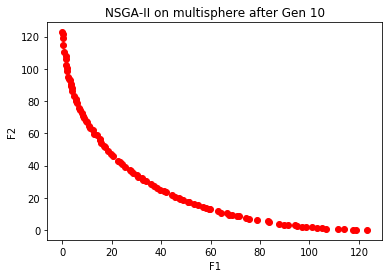
\includegraphics[width=0.9\linewidth]{../img/png/nsga2_verification.png}
	\caption{testrun of the NSGA-II algorithm on the multi-criteria sphere, shows the found solutions in function space}
	\label{fig:nsga2_verification}
\end{figure}



\section{Conjugate Gradient Descent}
\label{chap:cgd}
Compared to the previous algorithms, the Conjugate Gradient Method is a deterministic algorithm which uses a numeric approximation of the gradient. This method is again capable of optimising scalar valued functions. \\
The original idea dates back to \cite{hestenes_methods_1952}. It is specially constructed for optimising quadratic problems of the form $f(x) = \frac{1}{2}x^T H x + b^T x$. If the problem can be represented in this form, the CGD takes exactly $n$ iteration where $n$ is the dimensionality of the function $f: \mathbb{R}^n \rightarrow \mathbb{R}$. \\
The following pseudocode \ref{algo: CGD} outlines the implemented steps of the CGD. This algorithm also holds two subfunctions: \textit{numGrad} calculates the numeric gradient with the central differencing scheme and the \textit{linsearch} implements a golden section search starting from point $x$ and along a vector $d$. 

\begin{algorithm}
	\SetAlgoNoLine
	\DontPrintSemicolon
	$x$, $d$ $\gets$ initialization\;
	\While{$||\nabla f(x) || < \epsilon$ OR $||\hat{\eta}\textbf{d}|| < \epsilon$}
	{
		grad = numGrad(x)\;
		$\textbf{d}$ = $-grad$ + $\frac{||grad||^2}{||grad_{old}||^2 \textbf{d}}$\;
		\If {$\frac{grad\text{ }\textbf{d} }{||grad|| \text{ }||\textbf{d}||}$ > $-\alpha$} 
		{
			$\textbf{d}$ = -grad\;
		}
		$\hat{\eta}$ = linesearch(f(x, $\textbf{d}$))\;
		$x_{old}$ = x\;
		$grad_{old} = grad$\;
		$x = x + \hat{\eta} \textbf{d}$\;
	}
	\unterschrift{Conjugate Gradient Method}{}{}
	\label{algo: CGD}
\end{algorithm}


The plot in figure \ref{fig:CDG_verification} shows the function value per iteration of a CDG algorithm on a 2D sphere. As the sphere function is a quadratic function, the CDG is able to optimise it within the exact number of iterations as the dimension of the function. 


\begin{figure}[H]
	\centering
	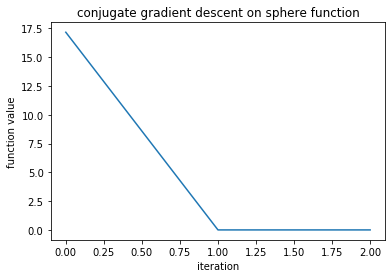
\includegraphics[width=0.9\linewidth]{../img/png/conjugate_gradient_descent_verification.png}
	\caption{testrun of the CDG algorithm on a 2D sphere}
	\label{fig:CDG_verification}
\end{figure}



\section{Hill Climbing}

The Hill Climbing method is a very simple from of optimisation algorithm. This method again optimises scalar valued problems. The general idea is to sample points around the current location, and select the new location based on the fitness values of these points. There are two main concepts, that need to be figured out to make the process work are: 
\begin{itemize}
	\item generating new solutions 
	\item stepsize adaption\\
\end{itemize}

In this implementation, new solutions are produced by going a step in positive and the negative direction of each coordinate. If two consecutive steps do not result in a better solution, the stepsize is adapted by bisecting it. The main issue with this method is, that it performs a strong local search and ultimately leads to a premature convergence. \\

The following pseudocode \ref{algo: HC} describes the necessary steps. 

\begin{algorithm}[H]
	\SetAlgoNoLine
	\DontPrintSemicolon
	$x_start$ $\gets$ initialization\;
	\While{fe < $\#FE_{max}$}{
		\For {d \textbf{in} Dim} 
		{
			z[d] = step\;
			$y_{1,2}$ = $x$ $\pm$ $step$\;
			f = funcion(y)\;
			fe = fe + 1\;
		}
		\If {function($y_d$) < function(x)} 
		{
			$x$ = $y_d$\;
		}
		\Else 
		{
			$step = 0.5 * step$ 
		}
		
	}
	\unterschrift{Hill Climbing}{}{}
	\label{algo: HC}
\end{algorithm}

The figure \ref{fig:HC_verification} shows how the HC heuristic optimises the sphere function. It is clearly seen, that this algorithm needs many more steps for the same function than the DE or CDG algorithm. 

\begin{figure}[H]
	\centering
	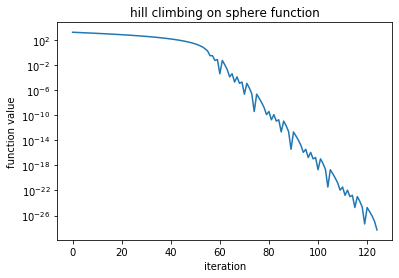
\includegraphics[width=0.9\linewidth]{../img/png/hill_climbing_varification.png}
	\caption{testrun of the HC heuristic on a sphere function}
	\label{fig:HC_verification}
\end{figure}


\chapter{Simulation Infrastructur}
The whole project is programmed in Python 3.7. The choice for that programming language was mainly that Sumo provides a rich API in Pyhton. Although the API is mainly designed to be used with Python 2.7, all necessary features also work in Pyhton 3. \\

All optimisation algorithms take a function handler as an input, which acts as the function to be optimised. In this case this is the Sumo simulation. Two versions of simulation function are created: a single- and a multi-criteria function. The multi-criteria function returns the three parameters ``stop count'' (sC in equation \ref{eq:stopcount}), ``waiting time'' (wT in equation \ref{eq:waitingtime}) and ``fairness'' (F in equation \ref{eq:fairness}) as a tuple. The waiting time is calculated by the mean over all waiting times for every car in the simulation. Similar the stop count is the sum of all stops in the whole simulation, but without normalisation of the number of cars. The fairness is defined as the variance over all waiting times meaning a smaller fairness results in a better fitness value. \\

Only the NSGA-II can handle these values separately. For all other algorithms, the single-criteria function is used. The three parameters are intermingled by a weighted mean (as seen in equation \ref{eq:singleCrit}). For the sake of simplicity, the weights are kept at 1. These three parameters can be read from the tripinfo file, which is automatically created by Sumo after every simulation.\\

\textbf{\underline{Problem:}} Since the cars can take a turn at every intersection, it might be possible that car gets trapped in the grid for a longer period. This artificially increases the number of stop counts and the waiting time. The optimiser can not improve this situation because the traffic light has no impact on this issue. To prevent that this effect weakens the found solutions, the function evaluation must be adapted. This is done by normalising the waiting time as well as the stop count with the length of the trip (rL) by that specific car. However, this also implies, that the grid is equally spaced. \\

\begin{equation}
wT = \frac{1}{N} \sum_{c = 0}^{N} \frac{wT_c}{rL}
\label{eq:waitingtime}
\end{equation}


\begin{equation}
sC = \sum_{c = 0}^{N} \frac{sC_c}{rL}
\label{eq:stopcount}
\end{equation}


\begin{equation}
fair = \frac{1}{N} \sum_{c = 0}^{N} (wT_c - wT)^2
\label{eq:fairness}
\end{equation}


\begin{equation}
singleCriteria = \frac{wWT \cdot wT + wSC \cdot sC + wF \cdot F}{wWT + wSC + wF}
\label{eq:singleCrit}
\end{equation}

Since this simulation is haevily subjected to randomness, one simulation would not be meaningful. Thus, a mean over 10 replications is calculated. \\

The following flowchart in \ref{fig:simulation_flowchart} shows the necessary steps to execute a full experiment. The state ``do optimizer steps'' is a placeholder for all other steps done by the optimisation algorithm. \\

The individuals are coded so that the problem to be optimised is 9-dimensional. On the first position of the vector is the cyclic time for a single traffic light. The following 8 parameters are the temporal offsets of each traffic light to the reference traffic light (counting from east to west).  

\begin{figure}[H]
	\centering
	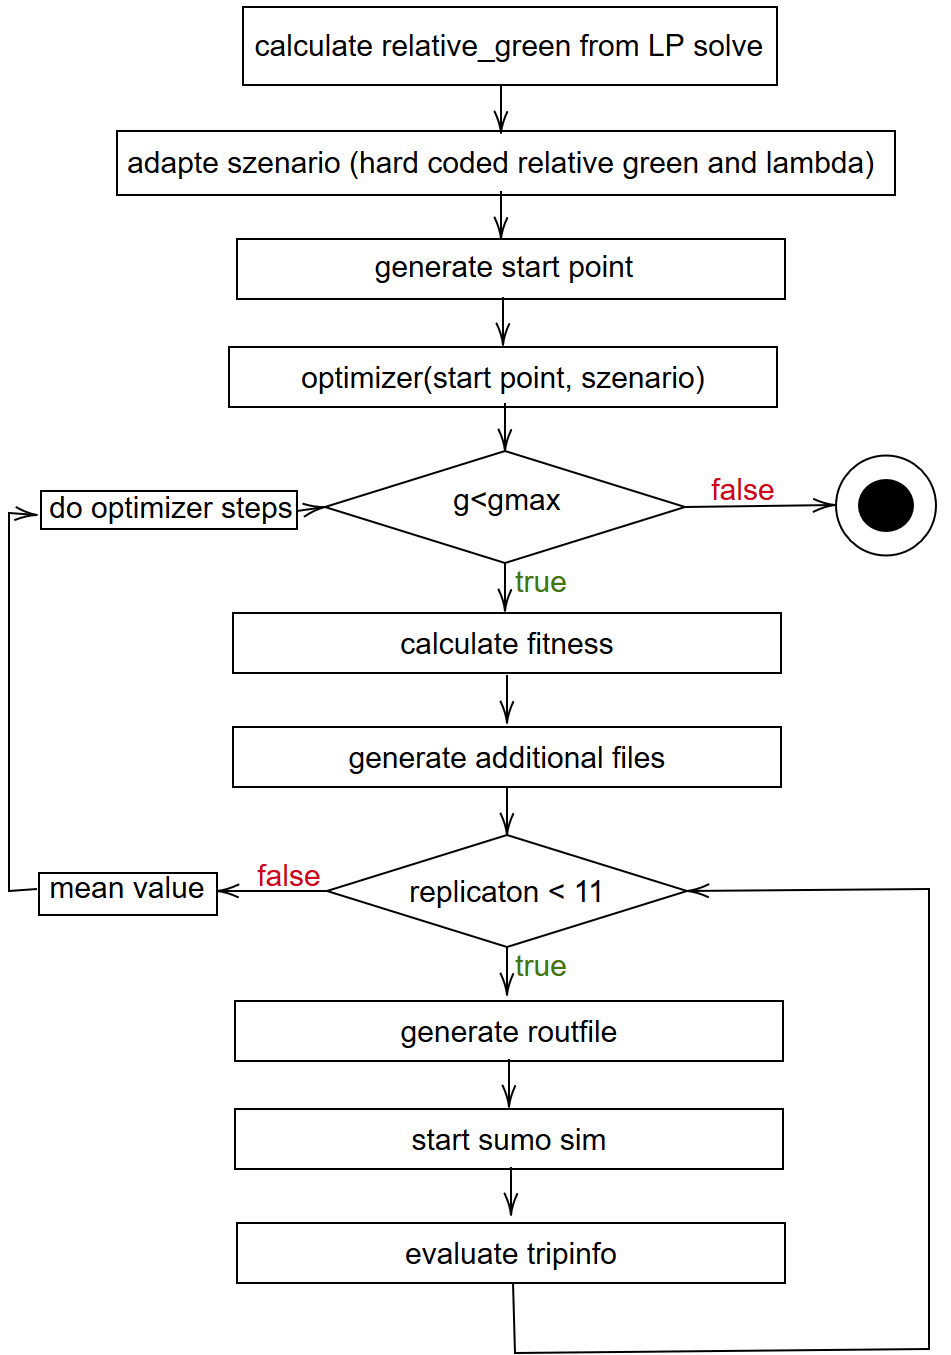
\includegraphics[width=\linewidth]{../img/png/simulation_flowchart.png}
	\caption{flowchart of a complete experiment including the setup and optimisation}
	\label{fig:simulation_flowchart}
\end{figure}



\chapter{Experiments}

This chapter describes all performed experiments. Since there are 4 optimisation algorithms and 2 scenarios, combining all results in 8 different experiments. These are described in the following chapters. 

\section{NSGA-II night}
The table \ref{tab:exp_nsga2_night} below shows the setup for this experiment. 
\begin{table}[H]
	\centering
	\noindent\adjustbox{max width=\linewidth}{
		\begin{tabular}{|c|c|}
			\hline
			\rowcolor[HTML]{\farbeTabA}
			Parameter & Value \\ \hline
			Population Size & 30\\ \hline
			Initialisation min & $\vec{x}^{\,T} = [5 \cdots 5]$ \\ \hline
			Initialisation max & $\vec{x}^{\,T} = [70 \cdots 70]$ \\ \hline
			Initialisation Strategy & uniform random \\ \hline
			Generation max & 15 \\ \hline
			Simulation time & 3600 steps = 1h \\ \hline
			Scenario layout & symmetric \\ \hline
			Replications & 10 \\ \hline
			Input Stream $\lambda$ & 0.0832499999999292 \\ \hline
			
		\end{tabular}
	}
	\unterschrift{parameter table of experiment NSGA-II at night}{}{}
	\label{tab:exp_nsga2_night}
\end{table}

The following two figures \ref{fig:exp_nsga2_night_result_g0} and \ref{fig:exp_nsga2_night_result_g14} show the distribution of the solutions in the function space. Without looking at the actual values, it can be concluded that the solutions tend to spread further apart with advancing number of generations. At the very least this proves that the NSGA-II algorithm is optimising the simulation. 

\begin{figure}[H]
	\centering
	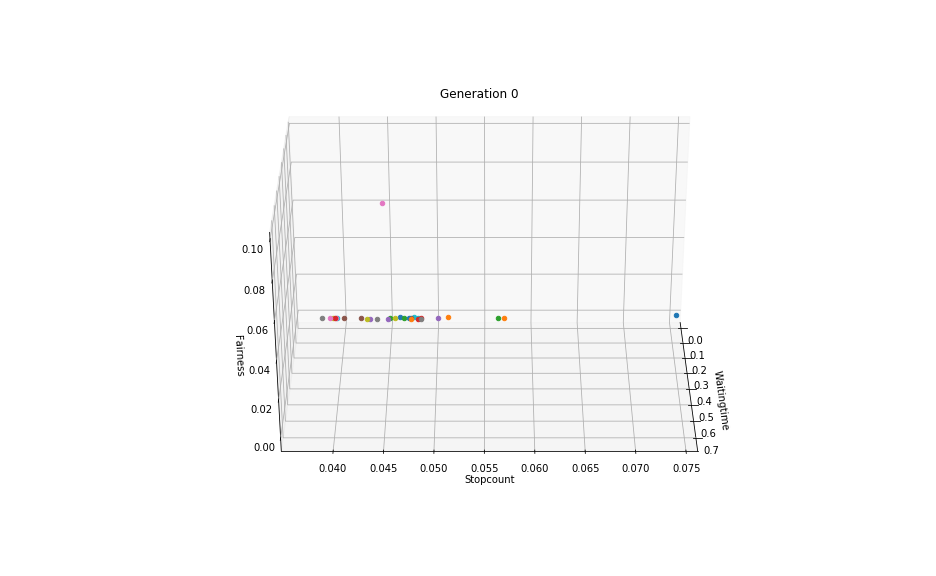
\includegraphics[width=\textwidth]{../img/png/nsga2_night_0.png}
	\caption{sample result of the NSGA-II on the night scenario after initialisation}
	\label{fig:exp_nsga2_night_result_g0}
\end{figure}


\begin{figure}[H]
	\centering
	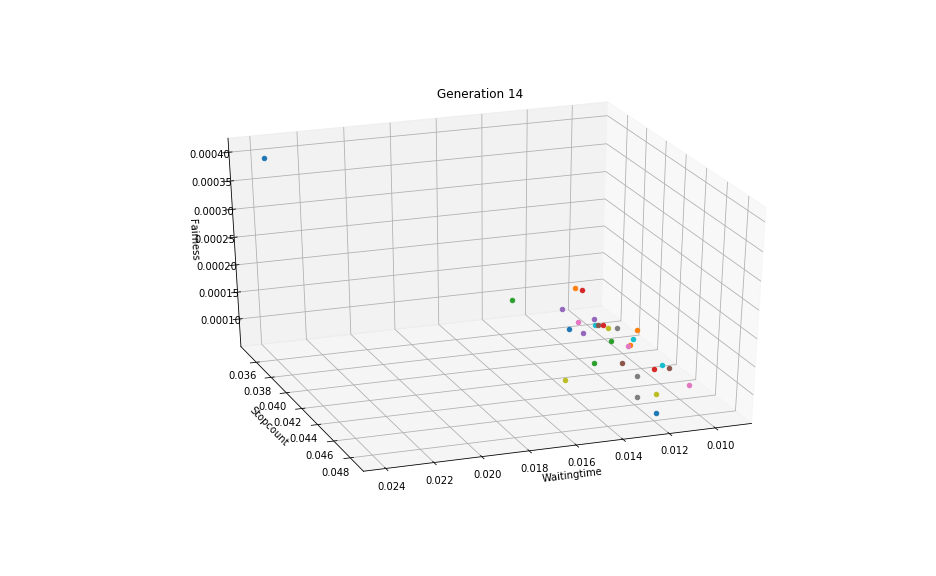
\includegraphics[width=\textwidth]{../img/png/nsga2_night_14.png}
	\caption{sample result of the NSGA-II on the night scenario after 14 generation}
	\label{fig:exp_nsga2_night_result_g14}
\end{figure}

\newpage

Figure \ref{fig:exp_nsga2_night_cycle_histo} shows the distribution of the optimised cycle time in the population. It can clearly be seen that the NSGA-II prefers smaller cycle times in the bin from 30 to 35. This is especially remarkable since the population was initialised uniformly random between 5 and 70. In a practical application the usefulness of such a short time is debatable: This only works if the cars drive nearly perfectly and start immediately after the light goes green without much of a reaction time.  


\begin{figure}[H]
	\centering
	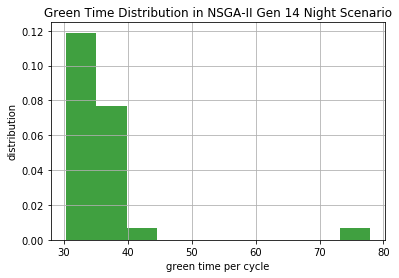
\includegraphics[width=\textwidth]{../img/png/nsga2_night_cycl_distr.png}
	\caption{Histogram of the cycle time distribution in the last population of the NSGA-II on the night scenarion.}
	\label{fig:exp_nsga2_night_cycle_histo}
\end{figure}

Looking at the offset times throughout the population is not very productive. These values are distributed between -78 and 161 and there is no way to draw any sensible conclusions from them. 


\section{NSGA-II day}

The table \ref{tab:exp_nsga2_night} below shows the setup for the experiment using an NSGA-II on the daytime scenario. In conjunction with the experiment on the night scenario, only the input stream and the maximum number of generations changed. 

\begin{table}[H]
	\centering
	\noindent\adjustbox{max width=\linewidth}{
		\begin{tabular}{|c|c|}
			\hline
			\rowcolor[HTML]{\farbeTabA}
			Parameter & Value \\ \hline
			Population Size & 30\\ \hline
			Initialisation min & $\vec{x}^{\,T} = [5 \cdots 5]$ \\ \hline
			Initialisation max & $\vec{x}^{\,T} = [70 \cdots 70]$ \\ \hline
			Generation max & 20 \\ \hline
			Simulation time & 3600 steps = 1h \\ \hline
			Scenario layout & symmetric \\ \hline
			Replications & 10 \\ \hline
			Input Stream $\lambda$ & 0.41625 \\ \hline
			
		\end{tabular}
	}
	\unterschrift{parameter table of experiment NSGA-II during the day}{}{}
	\label{tab:exp_nsga2_day}
\end{table}

Again, the following figures show the distribution of the population in the function space. Figure \ref{fig:exp_nsga2_day_result_g0} shows the population at generation 0. It is remarkable, that some solution cluster together and form groups at the stop count of 0, 5, 10 and 20. The population at generation 19 seen in figure \ref{fig:exp_nsga2_day_result_g19} clearly traces out a pareto front. 

\begin{figure}[H]
	\centering
	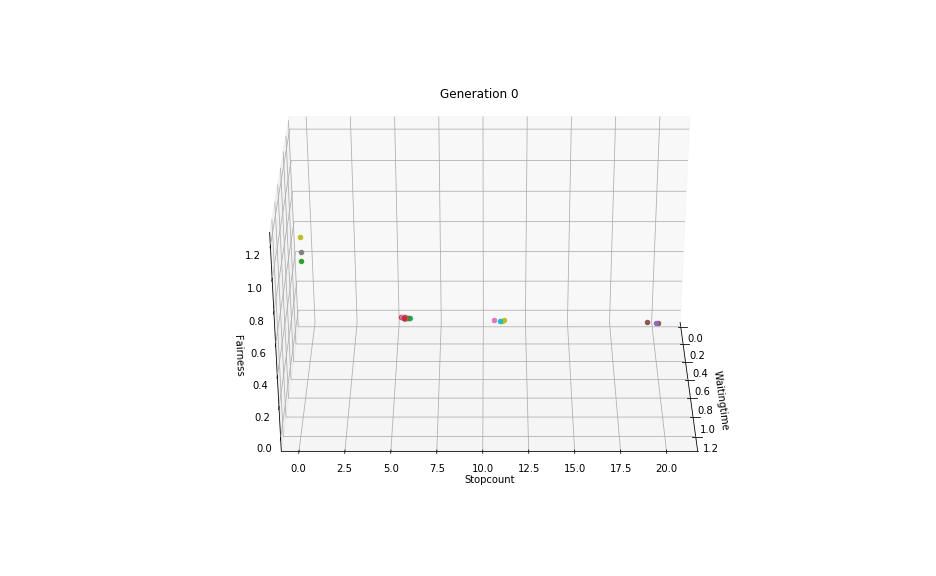
\includegraphics[width=\textwidth]{../img/png/nsga2_day_0.png}
	\caption{sample result of the NSGA-II on the day scenario after initialisation}
	\label{fig:exp_nsga2_day_result_g0}
\end{figure}


\begin{figure}[H]
	\centering
	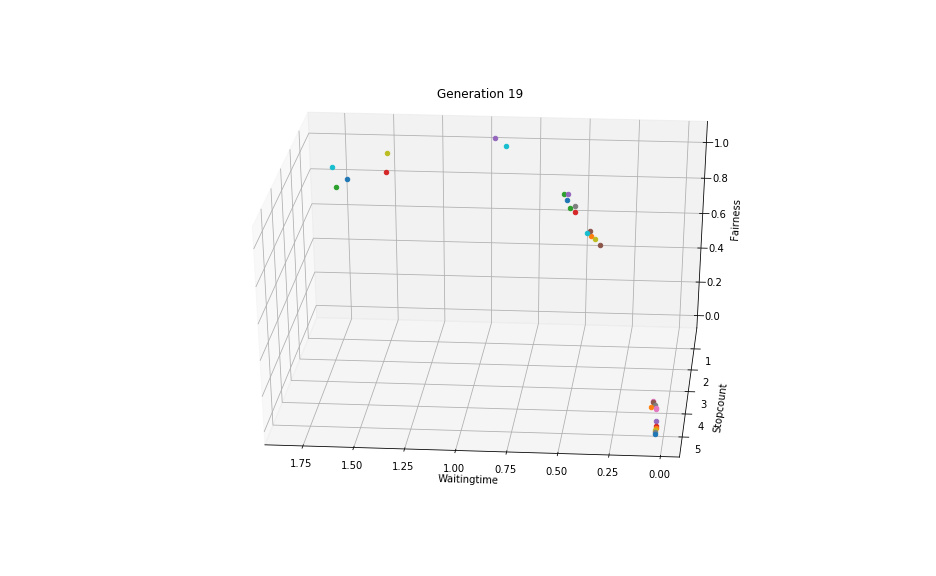
\includegraphics[width=\textwidth]{../img/png/nsga2_day_19.png}
	\caption{sample result of the NSGA-II on the day scenario after 19 generation}
	\label{fig:exp_nsga2_day_result_g19}
\end{figure}


Figure \ref{fig:exp_nsga2_day_cycle_histo} shows the distribution of the resulting cycle times in the last population. Most of the cycle times end up in the bin between 5 and 20. This again shows that the NSGA-II tends to grow towards shorter cycle times. 


\begin{figure}[H]
	\centering
	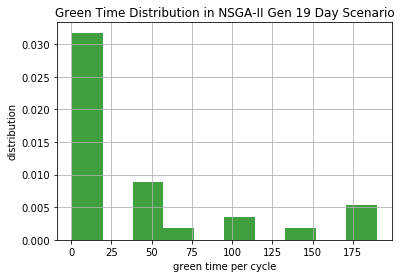
\includegraphics[width=\textwidth]{../img/png/nsga2_day_cycl_distr.png}
	\caption{Histogram of the cycle time distribution in the last population of the NSGA-II on the day scenarion.}
	\label{fig:exp_nsga2_day_cycle_histo}
\end{figure}

These values for the offset times are again very widely distributed between -107 and 189.  


\section{HC night}

The table below shows the parameter setup for running the HC algorithm on the night scenario. The starting point is initialised to a vector  $\vec{x}^{\,T}$ shown below. This point was chosen for two different reasons: 

\begin{itemize}
	\item it is already a pretty good solution; from there the algorithm should do the optimisation
	\item it is in middle of the last population found by the NSGA-II
\end{itemize}

This point servers as a the starting point for all other single-criteria algorithms. 

\begin{table}[H]
	\centering
	\noindent\adjustbox{max width=\linewidth}{
		\begin{tabular}{|c|c|}
			\hline
			\rowcolor[HTML]{\farbeTabA}
			Parameter & Value \\ \hline
			Initialisation & $\vec{x}^{\,T} = [90, 5, 10, 15, 20, 25, 30, 35, 40]$ \\ \hline
			Iteration max & 60 \\ \hline
			Step Size & 1 \\ \hline
			Simulation time & 3600 steps = 1h \\ \hline
			Scenario layout & symmetric \\ \hline
			Replications & 10 \\ \hline
			Weights & $[1, 1, 1]$ \\ \hline
			Input Stream $\lambda$ & 0.0832499999999292 \\ \hline
			
		\end{tabular}
	}
	\unterschrift{parameter table of experiment HC at night}{}{}
	\label{tab:exp_hc_night}
\end{table}

\newpage

The following plot in figure \ref{fig:exp_hc_night_result} shows how the function value decreases over time. The blue line denotes the explored function value in every direction, the orange line shows only the function values that have been improved. 

\begin{figure}[H]
	\centering
	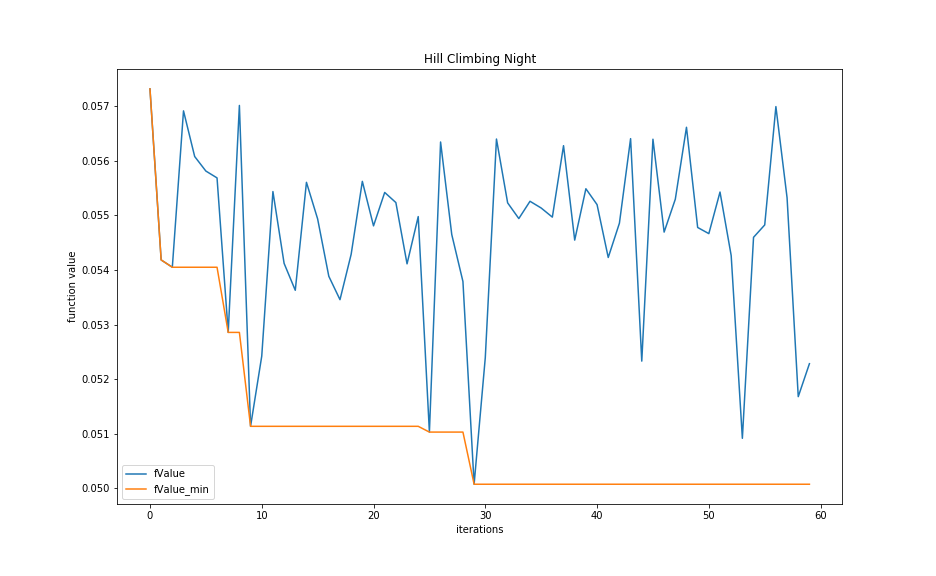
\includegraphics[width=\textwidth]{../img/png/hc_night.png}
	\caption{sample result of the HC Algorithm during the night scenario}
	\label{fig:exp_hc_night_result}
\end{figure}

The found optimum is located at vector seen in equation \ref{eq:hc_nigth_opt}. 
There is only very little change from the original starting point. This might depend on a various reasons: 

\begin{itemize}
	\item starting point was already near the optimum
	\item not enough iteration
	\item trapped in local optimum
\end{itemize}

\begin{equation}
f \left( \begin{bmatrix}
94.31268064 \\ -2.49787839 \\ 0.22650818 \\ 20.68603951 \\ 10.84759343 \\ 17.31755371 \\ 28.43479486 \\ 35.95338739 \\ 36.52319049
\end{bmatrix} \right) 
= 0.056852236013176254
\label{eq:hc_nigth_opt}
\end{equation}


\section{HC day}

Similar to the night scenario, the day scenario begins at the same starting point. Again the table \ref{tab:exp_hc_day} shows the experiment parameter. 

\begin{table}[H]
	\centering
	\noindent\adjustbox{max width=\linewidth}{
		\begin{tabular}{|c|c|}
			\hline
			\rowcolor[HTML]{\farbeTabA}
			Parameter & Value \\ \hline
			Initialisation & $\vec{x}^{\,T} = [90, 5, 10, 15, 20, 25, 30, 35, 40]$ \\ \hline
			Iteration max & 30 \\ \hline
			Step Size & 1 \\ \hline
			Simulation time & 3600 steps = 1h \\ \hline
			Scenario layout & symmetric \\ \hline
			Replications & 10 \\ \hline
			Weights & $[1, 1, 1]$ \\ \hline
			Input Stream $\lambda$ & 0.41625 \\ \hline
			
		\end{tabular}
	}
	\unterschrift{parameter table of experiment HC during the day}{}{}
	\label{tab:exp_hc_day}
\end{table}

The plot in figure \ref{fig:exp_hc_day_result} shows how the function value decreases over time. It is important to note, that the same starting point results in a greater function value compared to the night scenario. This must be correct since there are more cars in the system as compared to the night scenario. 

\begin{figure}[H]
	\centering
	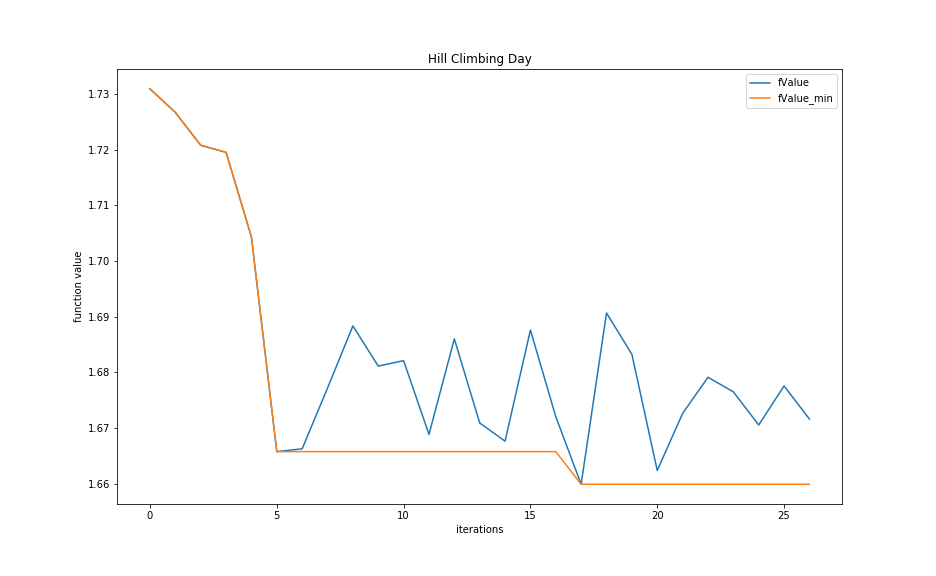
\includegraphics[width=\textwidth]{../img/png/hc_day.png}
	\caption{sample result of the HC Algorithm during the day scenario}
	\label{fig:exp_hc_day_result}
\end{figure}

The result is shown in the equation \ref{eq:hc_day_opt}. The cycle time of this optimum is smaller than the cycle time of the night scenario. This also checks out with the NSGA-II experiment where the cycle of the night scenario is greater than the one of the day scenario. 

\begin{equation}
f \left( \begin{bmatrix}
85.6798195 \\ 13.0753775 \\ 17.4374849 \\ 6.08137965 \\ 37.1726901 \\ 37.5230003 \\ 39.3042561 \\ 42.1506951 \\ 48.8756786
\end{bmatrix} \right) 
= 1.6746488062350436
\label{eq:hc_day_opt}
\end{equation}


\section{CGD on night and day}

As described above in \ref{chap:cgd} the CGD is especially helpful for quadratic functions. Since we have no idea of the form of this function, it is save to assume that the CGD is not very well suited for this problem. Further, the simulation is stochastic and thus the linesearch does employed along the gradient is results in a wrong stepsize. The following tables \ref{tab:exp_cgd_night} and \ref{tab:exp_cgd_day} show the parameter settings for both experiments. 

\begin{table}[H]
	\centering
	\noindent\adjustbox{max width=\linewidth}{
		\begin{tabular}{|c|c|}
			\hline
			\rowcolor[HTML]{\farbeTabA}
			Night Scenario & \\ \hline
			\rowcolor[HTML]{\farbeTabA}
			Parameter & Value \\ \hline
			Initialisation & $\vec{x}^{\,T} = [90, 5, 10, 15, 20, 25, 30, 35, 40]$ \\ \hline
			Stopping Criteria $\epsilon$ & 0.1 \\ \hline
			Safety Angle $\alpha$ & 0.1 \\ \hline
			Line Search $\eta$ & 10 \\ \hline
			Numeric Gradient $h$ & machine epsilon \\ \hline
			Simulation time & 3600 steps = 1h \\ \hline
			Scenario layout & symmetric \\ \hline
			Replications & 10 \\ \hline
			Input Stream $\lambda$ & 0.0832499999999292 \\ \hline
		\end{tabular}
	}
	\unterschrift{parameter table of experiment CGD at night}{}{}
	\label{tab:exp_cgd_night}
\end{table}


\begin{table}[H]
	\centering
	\noindent\adjustbox{max width=\linewidth}{
		\begin{tabular}{|c|c|}
			\hline
			\rowcolor[HTML]{\farbeTabA}
			Day Scenario & \\ \hline
			\rowcolor[HTML]{\farbeTabA}
			Parameter & Value \\ \hline
			Initialisation & $\vec{x}^{\,T} = [90, 5, 10, 15, 20, 25, 30, 35, 40]$ \\ \hline
			Stopping Criteria $\epsilon$ & 0.1 \\ \hline
			Safety Angle $\alpha$ & 0.1 \\ \hline
			Line Search $\eta$ & 10 \\ \hline
			Numeric Gradient $h$ & machine epsilon \\ \hline
			Simulation time & 3600 steps = 1h \\ \hline
			Scenario layout & symmetric \\ \hline
			Replications & 10 \\ \hline
			Input Stream $\lambda$ & 0.41625 \\ \hline
			
		\end{tabular}
	}
	\unterschrift{parameter table of experiment CGD during the day}{}{}
	\label{tab:exp_cgd_day}
\end{table}

In the resulting plots of the figures \ref{fig:exp_cgd_night_result} and \ref{fig:exp_cgd_night_result} it is clearly depicted that the CGD does not work for such a problem. Not only does the algorithm fails to optimise the function, it is also very computationally expensive: the numeric gradient must be calculated by taking the difference quotient in every direction. This already results in 18 function evaluation. Then the linesearch must be done which further increases the function evaluation count. 

\begin{figure}[H]
	\centering
	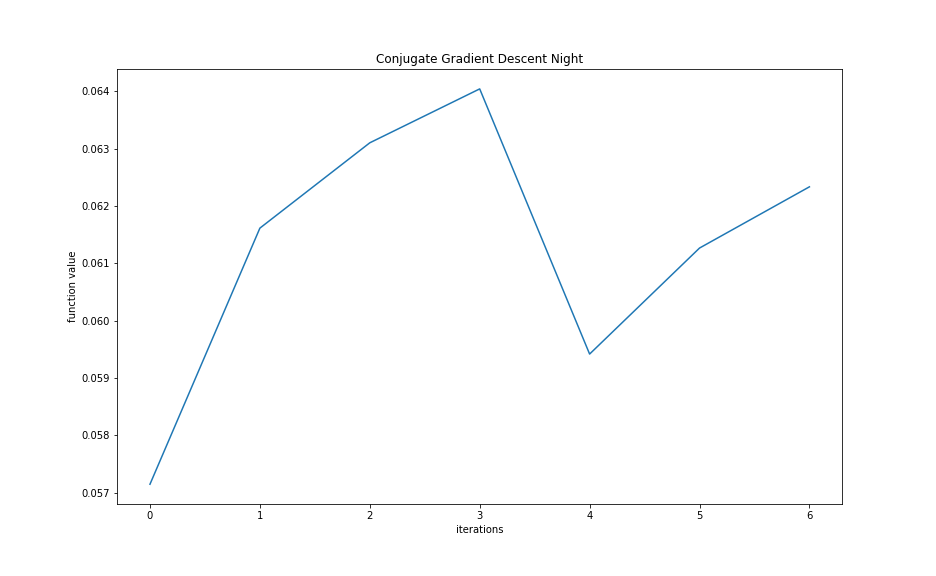
\includegraphics[width=\textwidth]{../img/png/cgd_night.png}
	\caption{sample result of the CGD Algorithm during the night scenario}
	\label{fig:exp_cgd_night_result}
\end{figure}


\begin{figure}[H]
	\centering
	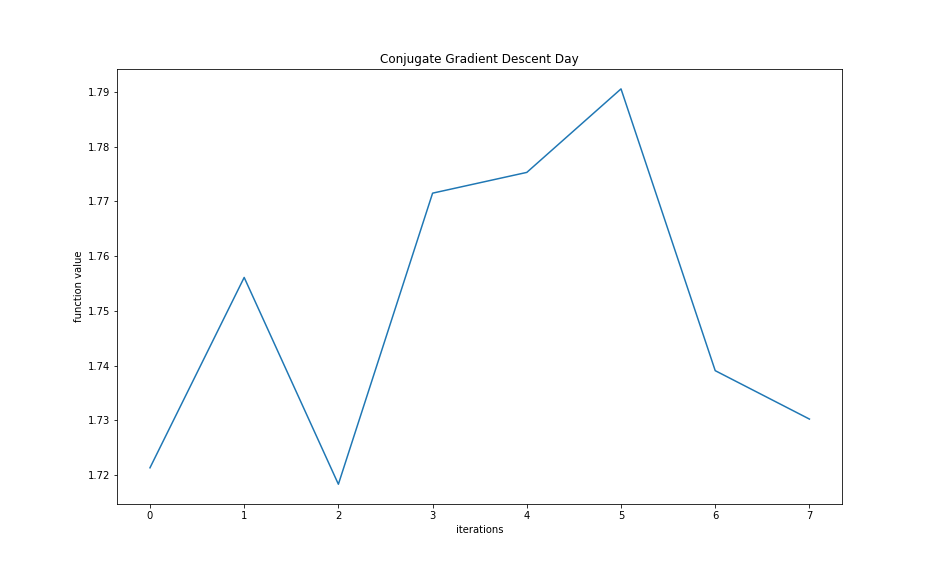
\includegraphics[width=\textwidth]{../img/png/cgd_day.png}
	\caption{sample result of the CGD Algorithm during the day scenario}
	\label{fig:exp_cgd_day_result}
\end{figure}

\newpage

\section{DE on night and day}

The tables below \ref{tab:exp_de_night} and \ref{tab:exp_de_day} below fully describe the parameter setting for the experiments. However, there have been a few issues with these experiments. 

\begin{table}[H]
	\centering
	\noindent\adjustbox{max width=\linewidth}{
		\begin{tabular}{|c|c|}
			\hline
			\rowcolor[HTML]{\farbeTabA}
			Night Scenario & \\ \hline
			\rowcolor[HTML]{\farbeTabA}
			Parameter & Value \\ \hline
			Population Size & 20\\ \hline
			Initialisation min & $\vec{x}^{\,T} = [5 \cdots 5]$ \\ \hline
			Initialisation max & $\vec{x}^{\,T} = [70 \cdots 70]$ \\ \hline
			Function Evaluation max & 10000 \\ \hline
			Mutation Operator & rand 1 \\ \hline
			Mutation Scale Factor $F$ & 0.5 \\ \hline
			Crossover Operator & binomial \\ \hline
			Crossover Probability & 0.1 \\ \hline
			Simulation time & 3600 steps = 1h \\ \hline
			Scenario layout & symmetric \\ \hline
			Replications & 10 \\ \hline
			Input Stream $\lambda$ & 0.0832499999999292 \\ \hline
			
		\end{tabular}
	}
	\unterschrift{parameter table of experiment DE at night}{}{}
	\label{tab:exp_de_night}
\end{table}


\begin{table}[H]
	\centering
	\noindent\adjustbox{max width=\linewidth}{
		\begin{tabular}{|c|c|}
			\hline
			\rowcolor[HTML]{\farbeTabA}
			 Scenario & \\ \hline
			\rowcolor[HTML]{\farbeTabA}
			Parameter & Value \\ \hline
			Population Size & 20\\ \hline
			Initialisation min & $\vec{x}^{\,T} = [5 \cdots 5]$ \\ \hline
			Initialisation max & $\vec{x}^{\,T} = [70 \cdots 70]$ \\ \hline
			Function Evaluation max & 10000 \\ \hline
			Mutation Operator & rand 1 \\ \hline
			Mutation Scale Factor $F$ & 0.5 \\ \hline
			Crossover Operator & binomial \\ \hline
			Crossover Probability & 0.1 \\ \hline
			Simulation time & 3600 steps = 1h \\ \hline
			Scenario layout & symmetric \\ \hline
			Replications & 10 \\ \hline
			Input Stream $\lambda$ & 0.41625 \\ \hline
			
		\end{tabular}
	}
	\unterschrift{parameter table of experiment DE during the day}{}{}
	\label{tab:exp_de_day}
\end{table}

\newpage

No results were gained in doing this experiment. The function evaluation (in this case the simulation) did not work correctly. Sumo experienced a lot of crashes and the DE algorithm could not even finish one generation. There might be a few reasons for that issue: 

\begin{itemize}
	\item The DE mutation operator \textbf{\textit{rand 1}} is known for spreading widely across search space as \cite{epitropakis_finding_2011} show in their paper. It is possible, that this operator generates a bad trail solutions that causes Sumo to crash.  
	\item There might be an error in the simulation function that has gone under the radar. However this is rather unlikely because the same functions was used for all other algorithms.  
\end{itemize}

\chapter{Critical Discussion}

A major issue that leads the CGD Algorithm to fail, might be the calculation of the numeric gradient. The tables \ref{tab:night_sensetivity} and \ref{tab:day_sensetivity} below show 10 different function evaluation for the day and night scenario where each result is already a mean over 10 replications. The stepsize for the difference quotient is the machine epsilon which is proven to be the best value. However, this number is so small, that it completly perishes in the stochastic effects of the simulation. Thus, the gradient does not necessarily point towards the highest increase. 


This effect could be minimised by using more replications. But since the experiments already take very long to calculate, this is not a productive measure. Another solution would be to take a bigger step and thus only look at the average change over a wider space. 


A different issue arises from the single-criteria function by calculating the weighted sum. The separate values for waiting time and fairness are relatively small compared to the big value of the stop count (depending on the solution this might be a factor between 100 and 1000). This means that the optimisation algorithm is more sensitive towards the stop count. If the algorithm should minimise all parameters equally, the weights must be adapted.  

\begin{table}[h]
	\centering
	\noindent\adjustbox{max width=\linewidth}{
		\begin{tabular}{|c|c|}
			\hline
			\rowcolor[HTML]{\farbeTabA}
			Run & Result \\ \hline
			1 & 0.05845304094188188 \\ \hline
			2 & 0.058203791618237855 \\ \hline
			3 & 0.06447016694180632 \\ \hline
			4 & 0.058089395318890756 \\ \hline
			5 & 0.05607968915837128 \\ \hline
			6 & 0.06045055736765529 \\ \hline
			7 & 0.059554536881858855 \\ \hline
			8 & 0.06064499410810244 \\ \hline
			9 & 0.061072665992490185 \\ \hline
			10 & 0.06496445913659102 \\ \hline \hline
			Mean & 0.060198329746588584 \\ \hline
			Variance & 7.084166340545999e-06 \\ \hline
			$f(x + h)$ & 0.05425510359003312 \\ \hline
			
		\end{tabular}
	}
	\unterschrift{results of 10 different runs on the night scenario}{}{}
	\label{tab:night_sensetivity}
\end{table}


\begin{table}[h]
	\centering
	\noindent\adjustbox{max width=\linewidth}{
		\begin{tabular}{|c|c|}
			\hline
			\rowcolor[HTML]{\farbeTabA}
			Run & Result \\ \hline
			1 & 1.7470391724996315 \\ \hline
			2 & 1.7903318700728446 \\ \hline
			3 & 1.734687539778108 \\ \hline
			4 & 1.7597643271768404 \\ \hline
			5 & 1.7526521713795522 \\ \hline
			6 & 1.7783639367329034 \\ \hline
			7 & 1.7603225664014694 \\ \hline
			8 & 1.7497671306402292 \\ \hline
			9 & 1.7328548281632024 \\ \hline
			10 & 1.7292531384605312 \\ \hline \hline
			Mean & 1.7535036681305312 \\ \hline
			Variance & 0.0003485028568951494 \\ \hline
			$f(x + h)$ & 1.7446520153831648 \\ \hline
			
		\end{tabular}
	}
	\unterschrift{results of 10 different runs on the day scenario}{}{}
	\label{tab:day_sensetivity}
\end{table}


\chapter{Conclusion and Further Work}

There are a few conclusions that could be drawn from the experiments: 

\begin{itemize}
	\item At first this might seem counterintuitive, but the experiments show that for the night scenario a greater cycle time is preferred as compared to the day scenario. 
	\item The NSGA-II works quite well for this problem. The experiments show that it optimises correctly, and it even traces out a (rudimentary) pareto front. 
	\item The Hill Climbing is the simplest of the tested algorithms. Although it takes longer for deterministic functions, it is very reliable on this kind of stochastic function. 
	\item The Conjugate Gradient Descent Algorithm does not optimise this function. This might be a consequence of 3 different issues: the small stepsize, the stochastic function and the need of a deterministic descent direction. 
	
\end{itemize}


During the project, several problems were encountered:  

\begin{itemize}
	\item Sumo is not very well documented, making the start not very gentle. The tutorials do not cover all the necessary parts for this project. This left us with a scrappy understanding of Sumo and its capabilities. 
	
	\item There is no possibility to evaluate the found results, except some self-constructed heuristic ideas. 
	
	\item Depending on the optimisation algorithm and the size of the problem, the computation time is very long (ranging from several hours to even days). Since Sumo is not installed on the school computers, this means that the students laptops are occupied for that time. This strictly limits the number of experiments that could be done. 
	
	\item Sometimes Sumo stops the simulation without any reasonable error. This means, that any running experiment must be started again with the last state. This further contributes to a temporal overhead. 
	
	\item During the simulation it is possible, that cars get teleported when the streets get crammed to much. This means that such a simulation is not accurate and must be disregarded. 
\end{itemize}


Further work could contain a renewed and optimised version of the simulation environment that takes less time to evaluate the function. This could be done by starting Sumo by a command line call, without going through the slower API communication which is done over TCP sockets. Further, the replications could be run in parallel to save even more time. \\
Although the parameters used are the ones that are typically recommended for these algorithms, the experiments could be redone by using different parameters. This might give a greater insight to which parameter are successful and how this particular problem is structured. 




\end{document}
